%!TEX root = ../../report.tex

\begin{figure}[H]
	\captionsetup[subfigure]{aboveskip=-0.8em,belowskip=0.5em}
	\newcommand{\figurewidth}{0.5\textwidth}
	\begin{subfigure}[b]{\figurewidth}
        \figureborder{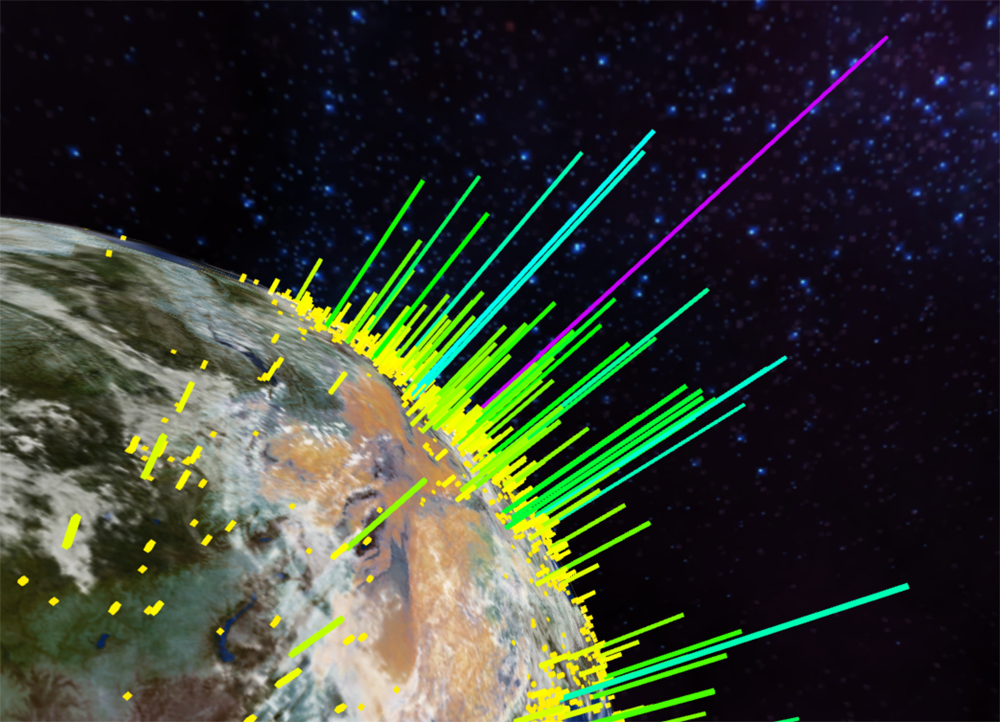
\includegraphics[width=\textwidth]{images/implementation/data_display/basic}}
		\caption{Basic shader display using a HSV colour range.}
		\label{fig:basic_shader}
	\end{subfigure}
	\begin{subfigure}[b]{\figurewidth}
		\figureborder{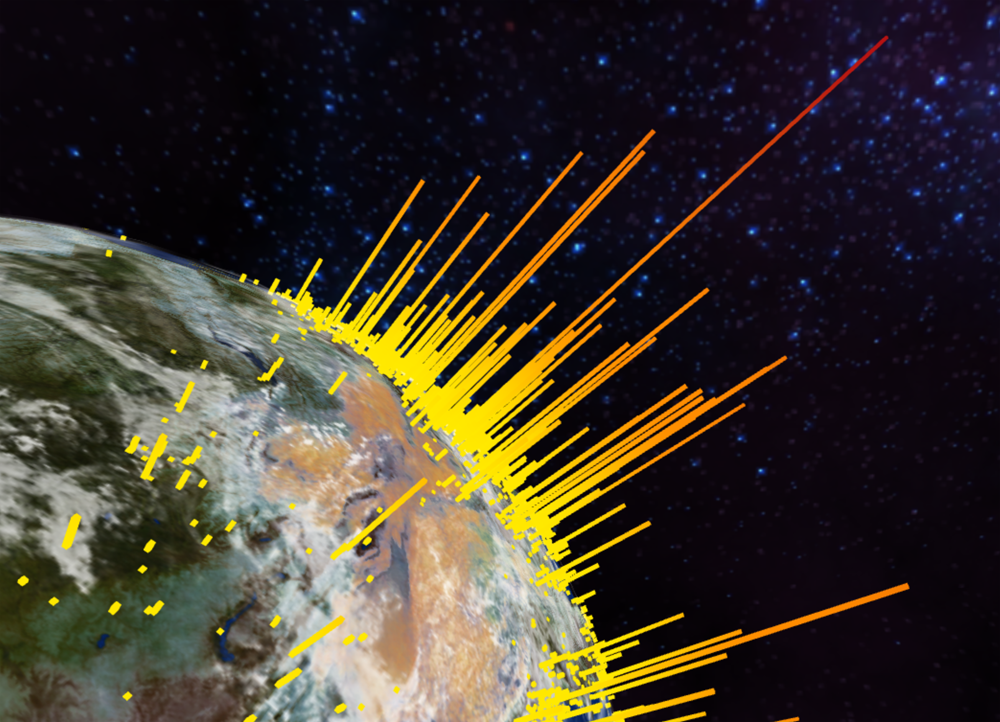
\includegraphics[width=\textwidth]{images/implementation/data_display/gradient}}
		\caption{Gradient shader data point display.}
		\label{fig:gradient_shader}
	\end{subfigure}
	\caption[Data point display types]{Types of data point displays.}
	\label{fig:data_point_displays}
\end{figure}
